\documentclass[11pt,a4paper]{article}
\usepackage[T1]{fontenc}
\usepackage{lmodern,amsmath,amssymb,amsthm,mathtools}
\usepackage[margin=25mm,headheight=16pt]{geometry}
\usepackage{graphicx,booktabs,longtable,array,tabularx}
\usepackage[dvipsnames]{xcolor}
\usepackage{microtype,enumitem,fancyhdr,needspace}
\usepackage[unicode=true,pdfencoding=unicode,colorlinks=true,linkcolor=MidnightBlue,citecolor=MidnightBlue,urlcolor=MidnightBlue]{hyperref}
\usepackage{bookmark}
\setlength{\parskip}{4pt}\setlength{\parindent}{0pt}
\setlength{\emergencystretch}{3em}\setlist{itemsep=2pt,topsep=4pt}
\allowdisplaybreaks[2]
\pagestyle{fancy}\fancyhf{}\fancyhead[L]{\small Measurement geometry}
\fancyhead[R]{\small Revision candidate v0.1.1}\fancyfoot[C]{\thepage}
\renewcommand{\headrulewidth}{0.3pt}
\newtheorem{theorem}{Theorem}[section]
\hypersetup{pdftitle={Measurement Geometry, Perspective, and Vesica Interfaces in the Tri-Octagon Model},pdfauthor={Hilmir Fr\'imann Halld\'orsson},pdfsubject={Revision candidate v0.1.1}}
\begin{document}
\begin{center}
{\small\color{MidnightBlue} TRI-OCTAGON MATHEMATICAL RESEARCH}\\[7mm]
{\LARGE\bfseries Measurement Geometry, Perspective, and Vesica Interfaces in the Tri-Octagon Model\par}\vspace{5mm}
{\large Hilmir Frímann Halldórsson}\\[3mm]
Revision candidate v0.1.1\\6 October 2026
\end{center}
\begin{abstract}
We give an exact account of the measurement geometry and adopted lens-to-state interface of the Tri-Octagon model. The width-one folded module is enclosed by the minimum centered vertical cylinder of radius \(1/\sqrt3\) and half-height \(1/2\). Its highest measurement ring is distinct from the nonplanar upper rim. Explicit projections separate normal, seam and tangent directions, and distinguish a measurement polygon from a regular reference hexagon. Historical changes of units are separated from fixed-centre changes of construction. For fixed nonzero extraction data, the lens initializer retains only the ratio \(d/r\); its fibres are positive scaling rays. Ratio recovery from amplitude is sharply Lipschitz, while angle recovery at tangency is Hölder. Deterministic vector error and finite-transfer attenuation explain conditioning without restoring absent absolute scale. Conditional enclosing hosts are retained in appendices. The cylinder is a static measurement definition and the oriented lens remains a kinematic interface; neither is assigned a material or rotational law.
\end{abstract}
\noindent\textbf{Keywords:} folded geometry; measurement scaffold; lens identifiability; inverse conditioning; SRG preparation\par
\vspace{3mm}
\textbf{Principal results and hypotheses.}
Lengths use the current octagon width as one. With the fixed centre and vertical axis, \(R_{\min}=1/\sqrt3\), \(H_{\min}=1/2\) (Section 3).
For known fixed \(v\ne0\), \(\Omega_0=Gv\) determines \(q=d/r\), but not \(r\); each fibre is \(\{(r,qr):r>0\}\) (Section 6).
The inverse obeys \(|Q(t_1)-Q(t_2)|\le\pi|t_1-t_2|\), whereas \(\theta(t)\sim(3\pi/4)^{1/3}t^{2/3}\) at tangency (Section 7). If \(v=0\), the whole lens domain collapses.

\textbf{Notation.} \(S\): folded surface; \(o\): centre; \(R,H\): cylinder radius and half-height; \(r,d\): lens radius and separation; \(q=d/r\); \(t=G\): amplitude gain; \(v\): fixed extracted vector. Appendix C gives the full crosswalk. Master labels M1--M38 and MA1--MA9 are retained.
\clearpage
\begingroup\small\setcounter{tocdepth}{1}\tableofcontents\endgroup
\clearpage
\section{The picture and the question}

The present construction consists of a fixed, folded polygonal surface and a surrounding coordinate scaffold. The owner's TL4 clarification gives the scaffold a precise purpose: the cylinder and its highest circular ring are \textbf{measurement geometry}, enclosing the centre and the entire Tri-Octagon. They have no specified material response or evolution. A separate Vesica-derived eye may eventually be oriented relative to this frame, but no rotation law has been supplied.

That clarification changes the mathematical question. An enclosing reference cylinder can be specified from exact coordinate extrema; selecting a material host would additionally require a choice of surface, attachment, and physical law. Earlier TL3 calculations explored conditional hosts. Their containment formulas remain valid, but none is needed to define the measurement cylinder, and none was adopted as material physics.

The resulting account has two parts. First, which lengths, directions, and projected outlines are actually supplied by the folded module? Second, which lens information reaches the canonical initial state through the existing adopted initializer? The first determines a reference frame. The second is an identifiability and conditioning problem. Neither supplies dynamics for a surrounding eye.

\textbf{Definition/\allowbreak{}adoption and source boundary.} TL4's meaning of \textquotedblleft{}top circle\textquotedblright{} is a current owner clarification. TL0's earlier historical recovery remains \textbf{TOP\_\allowbreak{}CIRCLE\_\allowbreak{}DISTINCT\_\allowbreak{}OBJECT = OPEN /\allowbreak{} NOT\_\allowbreak{}FORMALIZED}: the clarification does not retrospectively identify every historical ring or drawing. No NASA attribution, missing DMQPF explanation, or physical interpretation is inferred from recollection. [TL0 \S{}\S{}1--9; TL4 \textquotedblleft{}Scope and evidence.\textquotedblright{}]

\section{The exact width-one folded module}

All lengths below use the current flat-to-flat octagon width as one unit. This is a geometric normalization, not a calibrated physical length. Put

\[
s=\sqrt2-1,\qquad a=\frac12,\qquad p=\frac1{2\sqrt3},
\qquad o=(0,\sqrt3/6,0),\qquad e_z=(0,0,1).
\tag{M1}\label{eq:M1}
\]

Here \(s\) is an octagon side, \(a\) its apothem and vertical half-height, \(p\) the distance from the symmetry centre \(o\) to a face centre. These are different lengths. The local filled octagon has vertices

\[
\begin{gathered}(-1/2,-s/2),(-s/2,-1/2),(s/2,-1/2),(1/2,-s/2),\\
(1/2,s/2),(s/2,1/2),(-s/2,1/2),(-1/2,s/2).\end{gathered}
\tag{M2}\label{eq:M2}
\]

In the source's material coordinates \((u,z)\), its three affine panel maps at \(\beta=\pi/3\) are

\[
\begin{aligned}
P_1(u,z)&=(-1/2+(1/2-u)\cos\beta,(1/2-u)\sin\beta,z),\\
P_2(u,z)&=(u,0,z),\\
P_3(u,z)&=(1/2-(1/2+u)\cos\beta,(1/2+u)\sin\beta,z).
\end{aligned}\tag{M3}\label{eq:M3}
\]

Their union \(S\) is the union of the \textbf{filled panels}, with 18 welded vertices, three seams and two nonplanar nine-edge rims. There are no top or bottom caps. Twenty-four face-vertex incidences do not mean twenty-four different vertices.

For measurement, the centred face description is simpler. With face labels \(A=P_1,B=P_2,C=P_3\), define

\[
n_A=(-\sqrt3/2,1/2,0),\quad n_B=(0,-1,0),\quad
n_C=(\sqrt3/2,1/2,0),\qquad t_i=e_z\times n_i.
\tag{M4}\label{eq:M4}
\]

Each face centre is \(c_i=o+pn_i\). As a point set, its panel is exactly

\[
x-o=pn_i+ut_i+ze_z,\qquad |u|\le\frac12,
\quad |z|\le U(u):=\min\left(\frac12,\frac1{\sqrt2}-|u|\right).
\tag{M5}\label{eq:M5}
\]

The material sign of \(u\) in \eqref{eq:M3} need not agree on every face with the tangent-oriented \(u\) in \eqref{eq:M5}; the polygonal sets agree.

\textbf{Derived identity.} Write \(\rho=\|(I-e_ze_z^T)(x-o)\|\). Orthogonality of the frame gives

\[
\rho^2=p^2+u^2,\qquad p\le\rho\le\frac1{\sqrt3},
\qquad |z|\le\frac12.
\tag{M6}\label{eq:M6}
\]

Every vertex has the same centred squared norm

\[
B^2=p^2+\frac14+\frac{s^2}{4}
=\frac{13}{12}-\frac{\sqrt2}{2}.
\tag{M7}\label{eq:M7}
\]

The high vertices have \((\rho,|z|)=(v_6,1/2)\), where \(v_6=\sqrt{5/6-\sqrt2/2}\simeq0.355283763\); seam vertices have \((\rho,|z|)=(1/\sqrt3,s/2)\). The largest horizontal radius occurs below the top plane. A circle fitted only to the top vertices would miss the seams. [Inherited geometry: native geometry.py and face\_\allowbreak{}state.py; TL3 \S{}2, (1)--(3); TL4 \textquotedblleft{}Sharp enclosure.\textquotedblright{}]

\section{Measurement cylinder and highest ring}

\textbf{Conditional measurement definition.} Fix the centre \(o\) and vertical axis \(o+\mathbb R e_z\). For \(R,H>0\), let

\[
\boxed{C(R,H)=\{x:\rho\le R,\ |z|\le H\}},\qquad
z=(x-o)\cdot e_z.
\tag{M8}\label{eq:M8}
\]

Here \(H\) is \textbf{half-height}; the full height is \(2H\). Set \(e_x=(1,0,0)=t_B\), \(e_y=(0,1,0)\). Its highest circular ring is

\[
\boxed{\Gamma_+(R,H)=
\{o+R(\cos\psi\,e_x+\sin\psi\,e_y)+He_z:0\le\psi<2\pi\}.}
\tag{M9}\label{eq:M9}
\]

The solid cylinder's full maximum-height set is a disk. The owner's top ring is that disk's circular boundary, not the entire disk, the lateral surface, or the vertical axis.

\textbf{Exact theorem, fixed registration.} The complete panel surface satisfies

\[
\boxed{S\subset C(R,H)\quad\Longleftrightarrow\quad
R\ge R_{\min}=\frac1{\sqrt3},\quad H\ge H_{\min}=\frac12.}
\tag{M10}\label{eq:M10}
\]

To prove sufficiency, apply \eqref{eq:M6} to every panel point. Necessity follows because \(|u|=1/2\) is attained on seams and \(|z|=1/2\) on short horizontal edges. These independent extrema require both inequalities. The centre already lies in every such cylinder. Convexity also gives enclosure of \(\operatorname{conv}(S\cup\{o\})\), without declaring that convex hull a material core.

Thus the minimum radius is \(0.577350269\ldots\), diameter \(2/\sqrt3\), half-height \(1/2\), and full height 1. These minima are for the stipulated centred vertical cylinder; no optimization over tilted or displaced cylinders is asserted.

At equality the lateral surface touches the seams for \(|z|\le s/2\), while the top and bottom disks meet the short horizontal edges. The native shell does \textbf{not} touch the highest circular ring: at \(z=1/2\) its radius is at most \(v_6<1/\sqrt3\). Its upper rim contains six vertices at height \(1/2\) and three at \(s/2\). Three noncollinear high vertices fix the plane \(z=1/2\), excluding the other three, so that rim cannot be a Euclidean circle. A topological boundary cycle and a measurement circle are different objects. [TL0 \S{}6; TL4 (7)--(10), written sharpness proof.]

For an additional centred horizontal measurement polygon with largest vertex radius \(\rho_P\), placed at height \(z_0\), the joint enclosure is exactly

\[
R\ge\max(1/\sqrt3,\rho_P),\qquad
H\ge\max(1/2,|z_0|).
\tag{M11}\label{eq:M11}
\]

A planar footprint alone supplies no nonzero height. This applies separately to a chosen regular reference hexagon; it does not turn that hexagon into a shell section.

\begin{figure}[htbp]\centering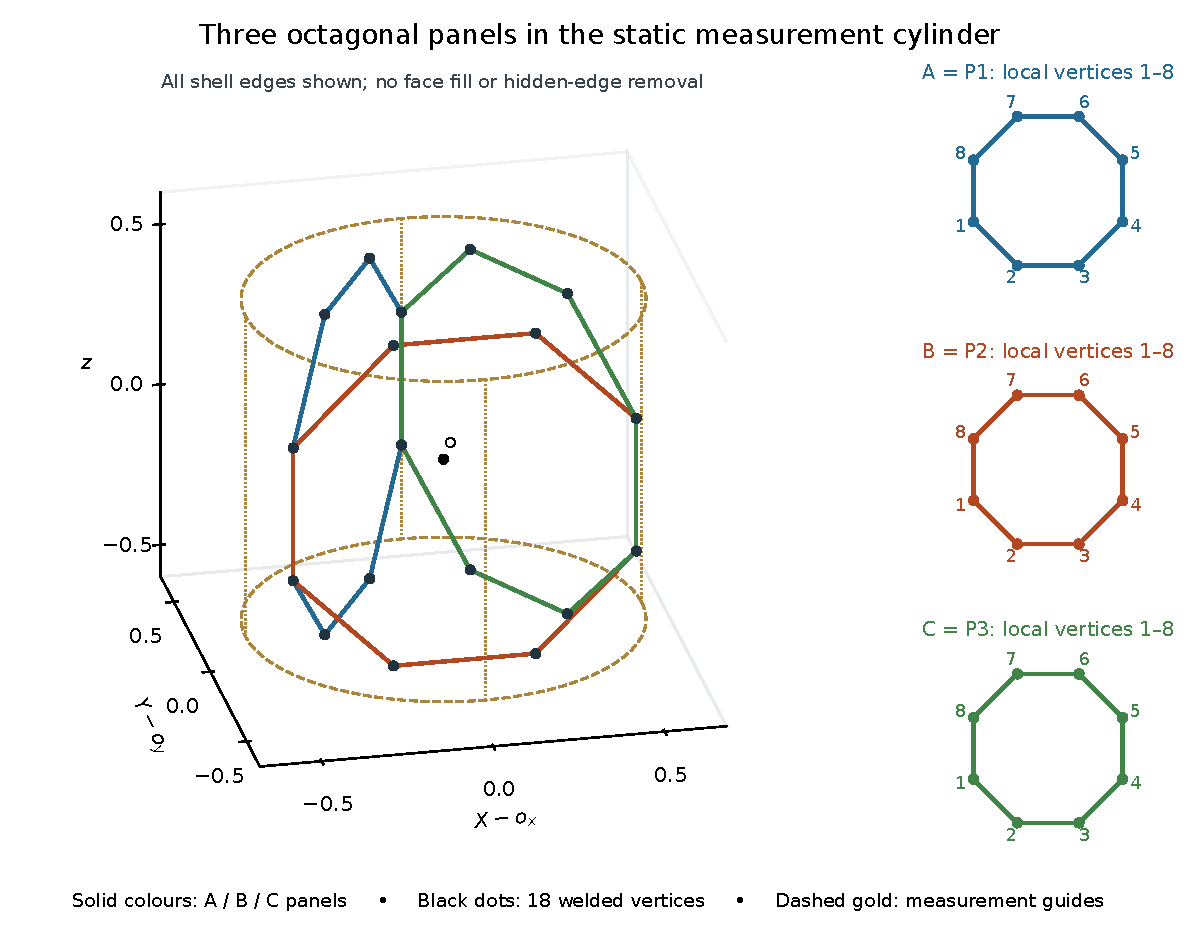
\includegraphics[width=\textwidth]{figures/scaffold.pdf}\caption{Exact coordinate construction in width-one units centered at \(o\), with \(R=1/\sqrt3\), \(H=1/2\). Left: all edges of the three octagonal panels, drawn without face fill or hidden-edge removal; black markers show the 18 welded vertices. The three seams are shared edges. Right: the eight ordered local vertices of each face, shown in material coordinates, not as a changed 3D arrangement. Dashed gold cylinder guides are measurement geometry, not shell edges. Equations (M1)--(M11); authoritative mesh rendering, no dynamics.}\label{fig:scaffold}\end{figure}

\section{Projections, directions, and the two hexagons}

\subsection{What a top view actually shows}

Top projection is \(\pi_z(x)=(e_x\cdot(x-o),e_y\cdot(x-o))\). In \eqref{eq:M5} it removes \(z\), leaving three complete segments \(pn_i+ut_i\), \(-1/2\le u\le1/2\). Hence

\[
\pi_z(S)=\text{the perimeter of an equilateral triangle of side 1}.
\tag{M12}\label{eq:M12}
\]

It is not a filled triangle or hexagon. The filled triangle is its convex hull. The highest subset projects to three short segments of length \(s\). Connecting their six endpoints by three additional measurement chords produces an alternating hexagon. Those extra chords are not edges of the native shell.

For comparison, a side view along the line \(n_B\), with screen \((t_B,e_z)\), retains \((x,z)\). Let \(U_z=\min(1/2,1/\sqrt2-|z|)\). The panels project at fixed \(z\) to

\[
[-U_z,U_z],\quad[-1/4-U_z/2,-1/4+U_z/2],\quad
[1/4-U_z/2,1/4+U_z/2].
\]

They overlap because \(U_z\ge s/2>1/6\). Their union proves

\[
\pi_{t_B,e_z}(S)=\{(x,z):|z|\le1/2,\ |x|\le1/4+U_z/2\}.
\tag{M13}\label{eq:M13}
\]

This is a filled nonregular octagon, with corners \((\pm1/2,\pm s/2)\) and \((\pm1/(2\sqrt2),\pm1/2)\). A triangle perimeter in one view and a filled octagon in another are consistent projections of exactly the same surface. [TL4 (12)--(18).]

\subsection{Directed rays are not unoriented axes}

Azimuths below run from \(+x=t_B\) towards \(+y\). A ray distinguishes \(v\) from \(-v\); the line \(\mathbb Rv\) does not.

\begingroup\small\setlength{\LTpre}{5pt}\setlength{\LTpost}{7pt}
\begin{longtable}{@{}>{\raggedright\arraybackslash}p{0.2500\dimexpr\textwidth-24pt\relax}>{\raggedright\arraybackslash}p{0.3700\dimexpr\textwidth-24pt\relax}>{\raggedright\arraybackslash}p{0.3800\dimexpr\textwidth-24pt\relax}@{}}
\toprule
\textbf{Object} & \textbf{Directed azimuths} & \textbf{Unoriented lines modulo \(180^\circ\)}\\ \midrule
\endfirsthead
\textbf{Object} & \textbf{Directed azimuths} & \textbf{Unoriented lines modulo \(180^\circ\)}\\ \midrule
\endhead
\bottomrule\endfoot
Face normals and face-centre rays & \(30,150,270^\circ\) & \(30,90,150^\circ\)\\[4pt]
Rays to projected seams; gap bisectors & \(90,210,330^\circ\) & Same normal lines\\[4pt]
Tangents \(t_i\) & \(0,120,240^\circ\) & \(0,60,120^\circ\)\\[4pt]
CCW connector directions & \(60,180,300^\circ\) & Same tangent lines\\[4pt]
Regular aligned hexagon vertex rays & \(0,60,120,180,240,300^\circ\) & Same tangent lines\\[4pt]
\end{longtable}\endgroup

The triangle corner opposite face \(i\) is \(-2pn_i\). Thus the seam-position rays are exactly \(-n_i\). The seam itself is a vertical segment: its spatial tangent is \(e_z\), not the horizontal ray to its projected point. Similarly \(\{R_{60}t_i\}=\{-t_i\}\). The normal and tangent line sets differ by \(30^\circ\) as unordered triples and are inequivalent under native \(D_{3h}\), although both are derived from the same frame. Three distinguished lines in a plane do not mean three independent coordinate dimensions.

For the aligned endpoint construction write

\[
A_i=pn_i-\frac{s}{2}t_i,\quad B_i=pn_i+\frac{s}{2}t_i,
\qquad g_{\rm gap}=\sqrt3p-\frac{s}{2}.
\tag{M14}\label{eq:M14}
\]

The selected edges have length \(s\); direct subtraction of adjacent endpoints gives connectors of length \(g_{\rm gap}\) in directions \(R_{60}t_i\). A regular hexagon requires

\[
g_{\rm gap}=s\quad\Longleftrightarrow\quad p=\frac{\sqrt3s}{2}.
\tag{M15}\label{eq:M15}
\]

For the current shell, \(g_{\rm gap}=s/\sqrt2\), so its top measurement hexagon is not regular. Its vertex rays have angles \(\alpha_i\pm\gamma\), where \(\alpha_i=\arg n_i\) and

\[
\gamma=\arctan\frac{s}{2p}
=\arctan(\sqrt3(\sqrt2-1))\simeq35.657130^\circ.
\tag{M16}\label{eq:M16}
\]

Only at regularity is \(\gamma=30^\circ\). The current endpoint rays must not be replaced by the regular hexagon's tangent-axis rays. The remembered \textquotedblleft{}three additional directions\textquotedblright{} could refer to opposite seam rays, opposite regular-hexagon rays, or tangent versus normal lines. Without a marked source, the intended choice remains open. [TL4 \textquotedblleft{}Top projection and the horizontal direction sets,\textquotedblright{} (14)--(15).]

\begin{figure}[htbp]\centering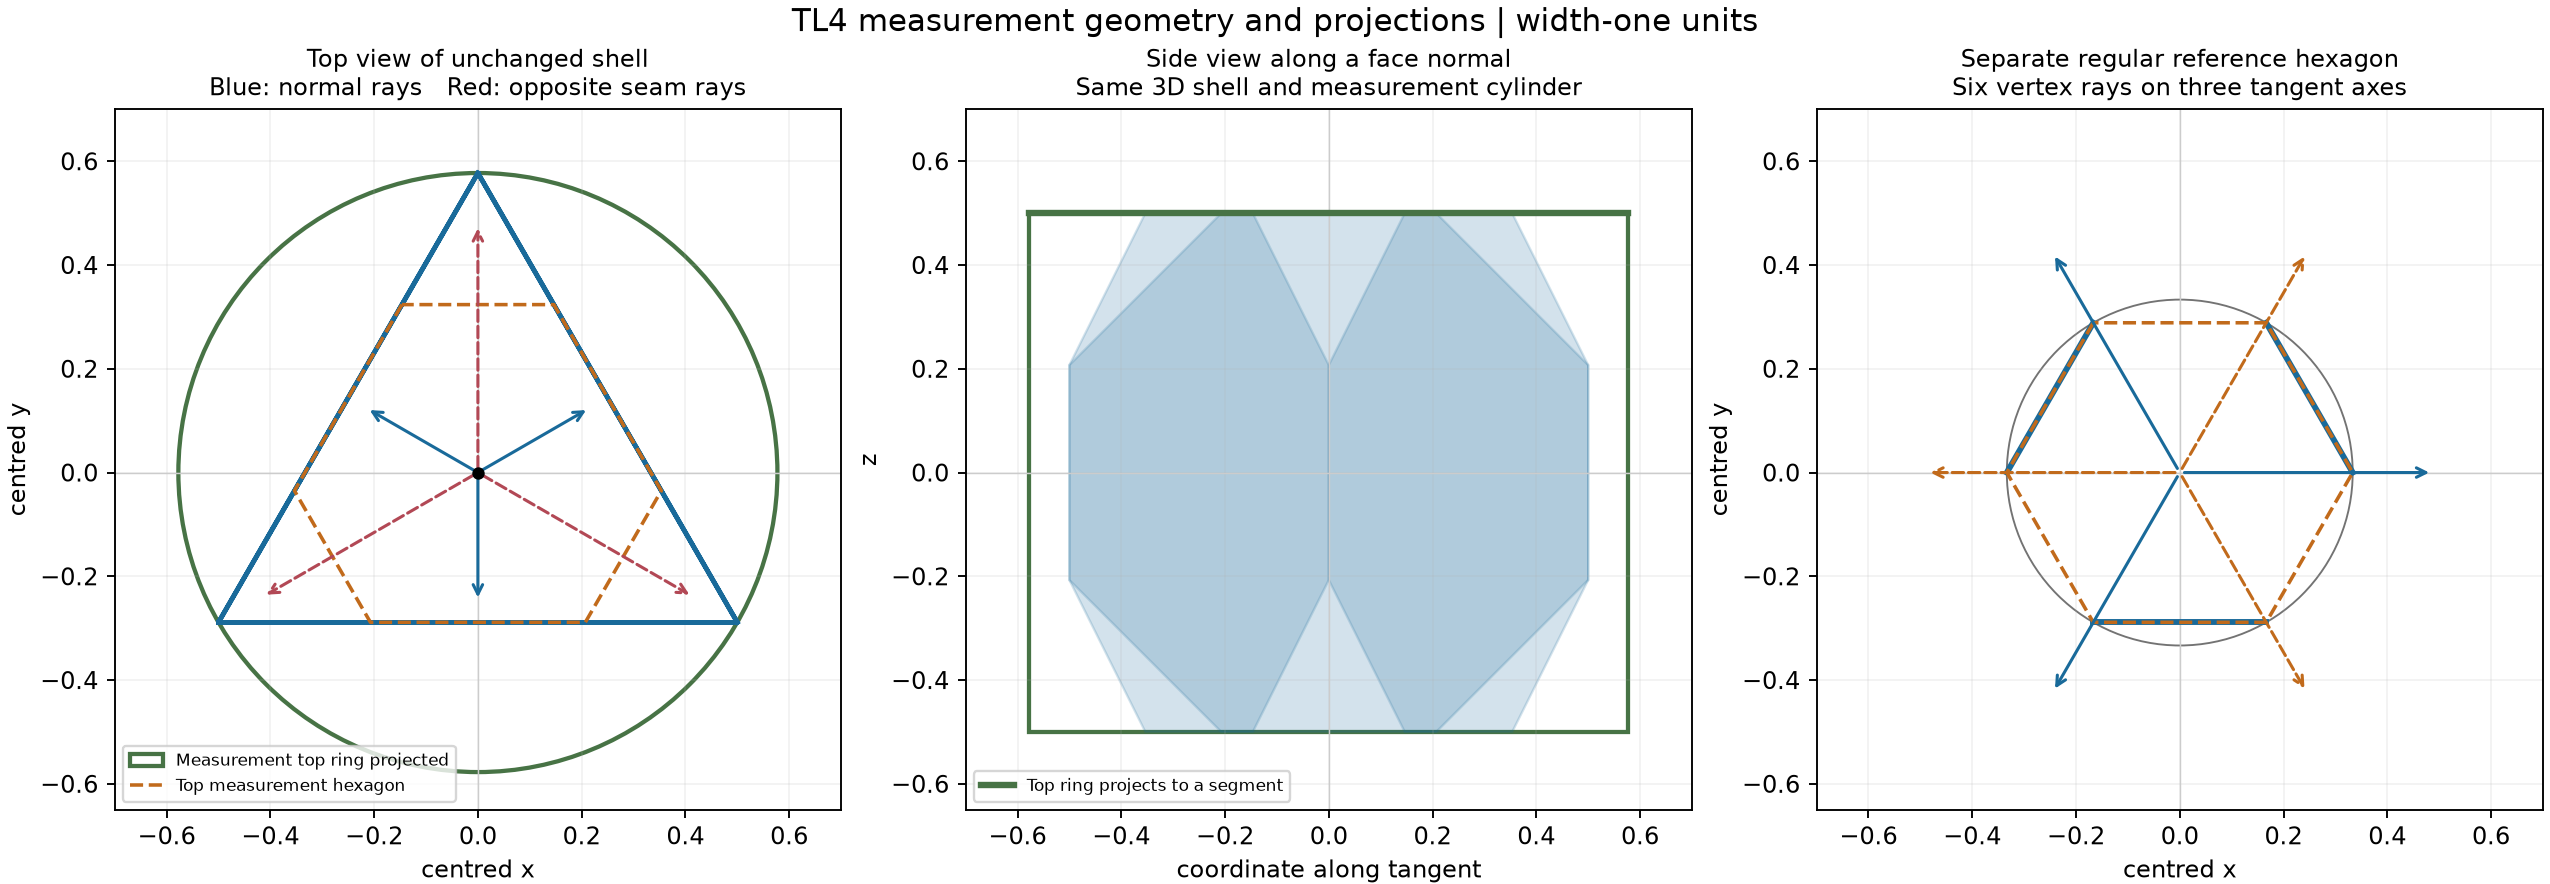
\includegraphics[width=\textwidth]{figures/TL4_MEASUREMENT_VIEWS.png}\caption{Retained TL4 static views in width-one coordinates: actual shell projections and a separate regular reference hexagon. Surface edges, measurement chords and reference geometry are distinguished by the original labels. Source: TL4, copied byte-for-byte; geometric diagram, not a dynamical simulation. Source hash in the supplement inventory.}\label{fig:tl4}\end{figure}

Left: triangle perimeter, alternating top measurement chain, and projected cylinder ring. Centre: side projection within the same measurement cylinder. Right: the distinct regular side-\(1/3\) reference hexagon. All three panels use the original width-one unit; the right panel is not a replacement for the welded shell.

\section{Normalization changes versus changes of construction}

The documented old folded export used octagon side \(s_{\rm old}=1\), hence width \(W_{\rm old}=1+\sqrt2\). The current export uses width one. The recovered relation, for corresponding coordinates about the same original origin, is

\[
\boxed{x_{\rm current}=(\sqrt2-1)x_{\rm old}.}
\tag{M17}\label{eq:M17}
\]

The symmetry centres obey the same scaling. Lengths scale by \(\sqrt2-1\), areas by \(3-2\sqrt2\); incidence and angles do not change. TL4 compared all 18 archived vertices. This conversion belongs to those documented folded exports, not arbitrary historical displays. [TL4 \textquotedblleft{}Two documented scales,\textquotedblright{} (1).]

\begingroup\small\setlength{\LTpre}{5pt}\setlength{\LTpost}{7pt}
\begin{longtable}{@{}>{\raggedright\arraybackslash}p{0.2500\dimexpr\textwidth-24pt\relax}>{\raggedright\arraybackslash}p{0.3700\dimexpr\textwidth-24pt\relax}>{\raggedright\arraybackslash}p{0.3800\dimexpr\textwidth-24pt\relax}@{}}
\toprule
\textbf{Quantity} & \textbf{Current width one} & \textbf{Old side one}\\ \midrule
\endfirsthead
\textbf{Quantity} & \textbf{Current width one} & \textbf{Old side one}\\ \midrule
\endhead
\bottomrule\endfoot
Octagon side & \(\sqrt2-1\) & 1\\[4pt]
Width/\allowbreak{}full height & 1 & \(1+\sqrt2\)\\[4pt]
Octagon apothem & \(1/2\) & \((1+\sqrt2)/2\)\\[4pt]
Individual octagon circumradius & \(\sqrt{1-\sqrt2/2}\) & \(\sqrt{4+2\sqrt2}/2\)\\[4pt]
Full-shell minimum cylinder radius & \(1/\sqrt3\) & \((1+\sqrt2)/\sqrt3\)\\[4pt]
\end{longtable}\endgroup

The separate fixed-face-centre matching operation holds \(p_0=a_0/\sqrt3\) fixed and shrinks each already placed face about its own centre. Its new side is \(\lambda_{\rm shrink}s_0\). Setting the connector equal to that side gives

\[
\sqrt3p_0-\lambda_{\rm shrink}s_0/2=\lambda_{\rm shrink}s_0,
\qquad
\boxed{\lambda_{\rm shrink}=\frac{1+\sqrt2}{3}.}
\tag{M18}\label{eq:M18}
\]

For initial width one, the resulting reference faces have side and connector \(1/3\), half-height \((1+\sqrt2)/6\), top hexagon circumradius \(1/3\), and whole-frame cylinder radius \(\sqrt{6+2\sqrt2}/6\). The operation loses the welded seams. It is not a change of units and does not describe the current shell.

An alternative retains the face size and translates each centre outwards to \(p_*=\sqrt3s/2\). Its whole-frame cylinder radius is \(\sqrt{(5-3\sqrt2)/2}\), half-height \(1/2\). The two regular alternatives are similar to each other by \eqref{eq:M18}, but not to the original folded arrangement. A global similarity preserves the original ratio \(g_{\rm gap}/s=1/\sqrt2\), so it cannot regularize that hexagon. [TL4 \textquotedblleft{}The hexagon matching calculation,\textquotedblright{} (4)--(6); inherited Paper D construction.]

The general reference scaffold uses \(p=(s+2g_{\rm gap})/(2\sqrt3)\), \(a=(1+\sqrt2)s/2\), and a different planar octagon-centre radius \(L=p+a\). Its Paper-C member is rigidly registered by

\[
M(x)=R_z(\pi/6)x+(0,a/\sqrt3,0),\qquad p=a/\sqrt3.
\tag{M19}\label{eq:M19}
\]

At \(s=\sqrt2-1\), no further scaling is needed. Reference indices \(0,1,2\) map to panels \(P_3,P_1,P_2\). Complete planar reference octagons and generic family members remain different point sets. Their radial bounds are \(\sqrt{(p+2a)^2+s^2/4}\) for complete planar frames and \(\sqrt{p^2+a^2}\) for complete vertical frames; the small hexagon only requires \(\sqrt{p^2+s^2/4}\). [TL4 reference registration (20) and footprint tables.]

\textbf{Distinct geometric quantities.} The documented individual-octagon circumradius \(0.541196100\ldots\) and full-shell cylinder radius \(0.577350269\ldots\) measure different extrema about different centres. Historical torus display values \(L=2,R_{\rm tube}=0.6\) instead give an envelope cylinder of radius 2.6 and half-height 0.6, with the torus's own highest circle at radius 2. No source fixes that display unit to the current width; their aspect ratios also prevent one similarity from matching both minimum-cylinder dimensions. [TL4 normalization and display tables.]

\section{The lens-to-state interface: shape without absolute scale}

The retained equal-radius planar lens has parent disks centred at \((\pm d/2,0)\), with \(r>0\), \(0\le d\le2r\). Its filled intersection is

\[
\mathcal L_{r,d}=\{(u,w):(|u|+d/2)^2+w^2\le r^2\}.
\tag{M20}\label{eq:M20}
\]

Set

\[
q=\frac dr\in[0,2],\qquad \theta=\arccos(q/2),\qquad
I(\theta)=\frac{2\theta-\sin2\theta}{\pi},\qquad G=\sqrt I.
\tag{M21}\label{eq:M21}
\]

The area is \(r^2(2\theta-\sin2\theta)\), so \(I\) is area divided by parent-disk area. The current named response lens\_\allowbreak{}area\_\allowbreak{}norm\_\allowbreak{}v1 adopts its square root as an amplitude gain. That adoption is not derived from a material aperture law.

Fix the incident vector \(\xi\in\mathbb C^2\), a named unit eigenbra \(\chi^\dagger\), and a finite preparation-transfer count \(n\ge0\). Writing \(n=3m+j\), \(j\in\{0,1,2\}\), the existing map is

\[
\boxed{\Omega_0=G(\theta)v},\quad
v=(\chi^\dagger\xi)b_\chi^n h_n f_j,\quad
h_n=D_s^m(1,q_s,q_s^2c_s)_j,
\tag{M22}\label{eq:M22}
\]

where \(\|f_j\|=1\), \(|b_\chi|=1\),

\[
q_s=e^{-.423},\quad r_s=e^{.577},\quad c_s=.382,\quad
D_s=r_sq_s^2c_s^2=e^{-.269}(.382)^2\in(0,1).
\tag{M23}\label{eq:M23}
\]

These decimal constants are the retained exact mathematical source constants. Their floating evaluation has its own contract. The count \(n\) is preparation, not the later nonlinear recurrence count; \(r_s\) is not a lens radius. No normalization of \(\Omega_0\) is inserted.

To make the factorization explicit, put \(\zeta_3=e^{2\pi i/3}\) and \(f_j=(1,\zeta_3^{-j},\zeta_3^{-2j})/\sqrt3\). The fixed spatial transfer \(A_s=R_sZ_sC_s\) acts by \(A_sf_0=q_sf_1\), \(A_sf_1=q_sc_sf_2\), \(A_sf_2=r_sc_sf_0\). Each complete three-step cycle therefore multiplies by \(D_s\); the remaining zero, one or two steps give the three factors in \eqref{eq:M22}. The full fixed transfer is \(U_s=B_s\otimes A_s\), with helicity-major tensor order. Applying the eigenbra to \(U_s^n[G(\xi\otimes f_0)]\) uses \(\chi^\dagger B_s^n=b_\chi^n\chi^\dagger\) and yields \eqref{eq:M22}. The named branches are negative\_\allowbreak{}imag and positive\_\allowbreak{}imag; their normalized eigenbra is fixed as part of the data. This is the existing SRG preparation, not the nonlinear recurrence. [TL1 \S{}1; native srg.py, fixed\_\allowbreak{}november\_\allowbreak{}srg, fourier\_\allowbreak{}basis and helicity\_\allowbreak{}mode.]

\begin{theorem}[Fixed-data fibres]\label{thm:fibres} Because \(q(\alpha r,\alpha d)=q(r,d)\),

\[
\Omega_0(\alpha r,\alpha d)=\Omega_0(r,d),\qquad \alpha>0.
\tag{M24}\label{eq:M24}
\]

Moreover \(I'(\theta)=4\sin^2\theta/\pi\). For any two distinct angles in \([0,\pi/2]\), the integral of this derivative between them is positive. Thus \(I\) and \(G\) are strictly increasing, including the endpoint where the derivative vanishes. They map onto \([0,1]\).

If \(v\ne0\), attainable outputs are exactly \(w=tv\), \(0\le t\le1\). The noiseless real scalar is \(t=v^\dagger w/\|v\|^2=\|w\|/\|v\|\). Hence \(\theta=I^{-1}(t^2)\) and \(q=2\cos\theta\) are unique. For that output the entire fibre is

\[
\{(r,d):r>0,\ d=q r\}
=\{(\alpha r_0,\alpha d_0):\alpha>0\}.
\tag{M25}\label{eq:M25}
\]

\end{theorem}
An output outside the segment has empty fibre. At \(t=1\), \(q=0\): all radii with \(d=0\) coincide. Here separation is known to be zero although radius is arbitrary. At \(t=0\), \(q=2\): the fibre is every tangency pair \((r,2r)\). Otherwise neither \(r\) nor \(d\) is individually recovered.

\textbf{Zero-output classification.} Every finite \(h_n\) is positive, all Fourier vectors are nonzero, and neither named eigenvalue vanishes. Explicitly \(b_\pm=\tau\pm i\sqrt{1-\tau^2}\), with \(\tau=\cos(2\pi\cdot.244)\cos(\pi\cdot.244)\) and \(|\tau|<1\). Therefore

\[
\Omega_0=0\quad\Longleftrightarrow\quad
d=2r\ \text{or}\ \chi^\dagger\xi=0.
\tag{M26}\label{eq:M26}
\]

Nonzero incidence does not guarantee nonzero extraction: for \(\chi=(a,b)\), the nonzero vector \((-\overline b,\overline a)\) is orthogonal to \(\chi\). If \(v=0\), the \textbf{whole} lens domain is one zero fibre and all nonzero-output fibres are empty. No branch/\allowbreak{}count-specific exact zero exists at finite \(n\) beyond these routes. Underflow, precision guards, and cancellation in binary64 are not additional exact mathematical fibres. [TL1 \S{}\S{}2--7; native boundary/\allowbreak{}SRG definitions.]

The interface forgets absolute common scale even in exact arithmetic. It also has no spatial orientation input. A proposed top-layer radius which matters independently cannot be identified through this initializer alone. This is an \textbf{information-interface result}, not a physical no-go theorem and not a reason to add a radius channel without adoption.

\section{Conditioning depends on the variable and error model}

Assume that \(v\) is fixed, known and nonzero. Write \(t=G\), \(Q(t)=q\), \(\Theta(t)=\theta\), and \(\delta(t)=2-Q(t)\). On the interior, differentiation gives

\[
\frac{dt}{d\theta}=\frac{2\sin^2\theta}{\pi t},\qquad
\frac{dt}{dq}=-\frac{\sin\theta}{\pi t},\qquad
\frac{dq}{dt}=-\frac{\pi t}{\sin\theta},\qquad
\frac{d\theta}{dt}=\frac{\pi t}{2\sin^2\theta}.
\tag{M27}\label{eq:M27}
\]

These are not endpoint substitution formulas. At coincidence \(q=0,t=1\), the respective last three derivatives have finite one-sided limits \(-1/\pi,-\pi,\pi/2\). At tangency their apparent \(0/0\) factors require asymptotics.

\subsection{Tangency asymptotics}

For \(\delta=2-q\to0^+\), the half-angle identity gives

\[
\theta=2\arcsin(\sqrt\delta/2)
=\sqrt\delta(1+\delta/24+3\delta^2/640+O(\delta^3)).
\]

Since \(dI/d\delta=\sqrt{4\delta-\delta^2}/\pi\), expanding and integrating from zero gives

\[
I=\frac4{3\pi}\delta^{3/2}
\left(1-\frac{3\delta}{40}-\frac{3\delta^2}{896}+O(\delta^3)\right),
\qquad
t=\frac2{\sqrt{3\pi}}\delta^{3/4}(1-3\delta/80+O(\delta^2)).
\tag{M28}\label{eq:M28}
\]

Define \(C_\theta=(3\pi/4)^{1/3}\), \(C_\delta=C_\theta^2\). Inversion in the fractional-power coordinate produces

\[
\delta(t)=C_\delta t^{4/3}+\frac{C_\delta^2}{20}t^{8/3}+O(t^4),
\quad
\Theta(t)=C_\theta t^{2/3}
\left(1+\frac{C_\delta}{15}t^{4/3}+O(t^{8/3})\right).
\tag{M29}\label{eq:M29}
\]

Thus \(Q\) and \(\delta\) are \(C^1\) at tangency, with derivative zero; their first derivatives have local Hölder exponent \(1/3\), and second derivatives diverge. Angle recovery is optimally Hölder \(2/3\), not Lipschitz or differentiable with finite derivative there. The forward gain is Hölder \(3/4\) as a function of \(q\). These exponents follow from the series, not fitted data. [TL2 \S{}3, (5)--(12).]

\textbf{Exact sharp bound.} On the whole gain interval,

\[
\boxed{|Q(t_1)-Q(t_2)|\le\pi|t_1-t_2|.}
\tag{M30}\label{eq:M30}
\]

Indeed

\[
\frac d{d\theta}\frac{I(\theta)}{\sin^2\theta}
=\frac{4(\sin\theta-\theta\cos\theta)}{\pi\sin^3\theta}\ge0.
\]

The numerator starts at zero and has derivative \(\theta\sin\theta\ge0\). The ratio reaches 1 at \(\pi/2\), so \(t\le\sin\theta\) and \(|Q'|\le\pi\). Integrating proves \eqref{eq:M30}; the slope at \(t=1\) proves sharpness. The same bound holds for \(\delta\). Absolute ratio recovery from amplitude is therefore not singular at tangency.

Relative condition numbers refer to \textbf{relative amplitude error}, \(\kappa_f=|t f'(t)/f(t)|\), when the denominator is nonzero:

\[
\kappa_\theta=\frac{2\theta-\sin2\theta}{2\theta\sin^2\theta},\quad
\kappa_q=\frac{2\theta}{\sin2\theta}-1,\quad
\kappa_\delta=\frac{2\theta-\sin2\theta}{2(1-\cos\theta)\sin\theta}.
\tag{M31}\label{eq:M31}
\]

Their tangency limits are \(2/3,0,4/3\); their coincidence limits are \(1,+\infty,\pi/2\). Relative errors of an exactly zero angle, gap, or ratio are undefined. If the datum instead has fixed \textbf{additive area error}, then \(\delta(I)\sim C_\delta I^{2/3}\), \(\Theta(I)\sim C_\theta I^{1/3}\), and \(|dq/dI|=\pi/(2\sin\theta)\to\infty\). This is a different inverse problem. Squaring an amplitude estimate induces area error \(2t\,e_t+e_t^2\), not an independent fixed area-error budget. [TL2 \S{}4, (13)--(16).]

\subsection{Arbitrary complex output error}

Let \(\widehat w=tv+e\), \(\|e\|\le\varepsilon_{\rm out}\), and \(V_0=\|v\|>0\). Minimizing \(\|\widehat w-sv\|^2\) over real \(s\) gives

\[
\widehat t=\frac{\operatorname{Re}(v^\dagger\widehat w)}{V_0^2},
\qquad |\widehat t-t|\le\frac{\|e\|}{V_0}
\le E_{\rm out}:=\frac{\varepsilon_{\rm out}}{V_0}.
\tag{M32}\label{eq:M32}
\]

The normal equation follows by differentiating a strictly convex quadratic in \(s\); the bound is Cauchy--Schwarz, sharp for real parallel error. If \(e=(a_e+ib_e)v+e_H\), \(v^\dagger e_H=0\), then \(\widehat t-t=a_e\). Both quadrature error \(ib_ev\) and Hermitian-orthogonal error leave that scalar estimate unchanged, although they contribute residual. Estimating \(t\) by \(\|\widehat w\|/V_0\) would not have this property.

Clipping the estimate to \([0,1]\) is nonexpansive relative to the true attainable \(t\). Thus

\[
|Q(\widetilde t)-Q(t)|\le\min(2,\pi E_{\rm out}).
\tag{M33}\label{eq:M33}
\]

This is estimator analysis, not an initializer change. If \(r_\perp=\widehat w-\widehat t v\), the exact feasible gain interval is

\[
\left[\widehat t-\frac{\sqrt{\varepsilon_{\rm out}^2-\|r_\perp\|^2}}{V_0},
\widehat t+\frac{\sqrt{\varepsilon_{\rm out}^2-\|r_\perp\|^2}}{V_0}\right]\cap[0,1],
\tag{M34}\label{eq:M34}
\]

provided the square root is real and the intersection nonempty. Otherwise the observation is incompatible with the error model. Applying decreasing \(Q\) reverses endpoint order.

In the resolved regime \(E_{\rm out}\ll t\ll1\), local errors scale as \((4/3)C_\delta t^{1/3}E_{\rm out}\) for the ratio/\allowbreak{}gap and \((2/3)C_\theta t^{-1/3}E_{\rm out}\) for the angle. These linearized estimates cannot be extrapolated to fixed error at \(t=0\). If \(t\le E_{\rm out}\), an admissible error can erase the output entirely. At true tangency the exact worst-case errors are \(\delta(\min(E_{\rm out},1))\) and \(\Theta(\min(E_{\rm out},1))\), hence asymptotically \(C_\delta E_{\rm out}^{4/3}\) and \(C_\theta E_{\rm out}^{2/3}\). A small gap can be unresolved relatively despite controlled absolute ratio error. [TL2 \S{}\S{}5--6, (17)--(23).]

\subsection{Extraction attenuation is a separate condition number}

Equation \eqref{eq:M22} gives \(V_0=|\chi^\dagger\xi|h_n\). Put \(p_0^{(s)}=1,p_1^{(s)}=q_s,p_2^{(s)}=q_s^2c_s\), \(\rho_s=D_s^{1/3}\). Then

\[
h_n=p_j^{(s)}\rho_s^{-j}\rho_s^n>0,\quad
h_{n+3}=D_sh_n,\quad
E_{\rm out}=\frac{\varepsilon_{\rm out}}{|\chi^\dagger\xi|h_n}.
\tag{M35}\label{eq:M35}
\]

Here \(D_s\simeq0.1115068404\), \(\rho_s\simeq0.4813199210\). Each three extra transfers multiplies fixed absolute-error amplification by \(D_s^{-1}\simeq8.96806\); the per-count asymptotic factor \(\rho_s^{-1}\simeq2.07762\) is not the ratio at every individual step. Every finite count remains exactly nonzero. This is attenuation, not exact information loss.

Likewise \(|\chi^\dagger\xi|\to0^+\) makes absolute-error amplification unbounded while preserving noiseless shape injectivity. At overlap exactly zero the whole-domain collapse \eqref{eq:M26} occurs. With a purely relative output budget \(\|e\|\le\varepsilon_{\rm rel}tV_0\), the extraction norm cancels and the local relative condition numbers apply. No stochastic assumption is used. No improvement in precision or gain can recover absolute \(r\), since different radii already have identical \textbf{noiseless} data. [TL2 \S{}\S{}7--8, (24)--(27).]

\section{Changing a view versus orienting the eye}

An orthonormal screen \(E=[a_0\ b_0]\), with sight direction \(c_0=a_0\times b_0\), gives coordinates \(E^T(x-o)\) and ambient projection \(I-c_0c_0^T\). For two points,

\[
\|E^T(x-y)\|^2=\|x-y\|^2-|c_0\cdot(x-y)|^2.
\tag{M36}\label{eq:M36}
\]

Depth and projected lengths change with the view; the object's distances do not. Top and side screens were used above. A face-on lens embedding is \(x=o+ua_0+wb_0\), with \eqref{eq:M20} in \((u,w)\).

To illustrate a quarter-turn without adopting a spin axis, conditionally take \(Q a_0=a_0\), \(Q b_0=c_0\), \(Q c_0=-b_0\). An active rotation changes the eye to \(o+ua_0+wc_0\) relative to the fixed scaffold. In its old screen it appears as \((u,0)\). A view change alone to screen \((a_0,c_0)\) makes the original fixed lens appear as \((u,0)\) as well. If object and screen rotate together,

\[
(QE)^TQ(x-o)=E^T(x-o).
\tag{M37}\label{eq:M37}
\]

The image is unchanged although the eye's relation to the fixed shell may have changed. A passive coordinate change applied to every object changes neither relation. These examples prove why a changed silhouette does not determine an active rotation. [TL4 (16)--(19).]

For a generic lens \(0<q<2\), an initial placement needs a plane \textbf{and} its in-plane centreline: a normal alone leaves one angle free. A marked right-handed frame \(Q=[a_0\ b_0\ c_0]\in SO(3)\) supplies three orientation degrees of freedom. For only the unlabeled lens set, half-turns about each frame axis preserve it, giving \(SO(3)/D_2\), with \(D_2\) the four-element group of those proper rotations. At \(q=0\), a disk needs only its plane, represented by an unoriented normal in \(\mathbb{RP}^2\). At \(q=2\), the overlap point has no orientation; the retained parent pair would still have one.

Polar coordinates and rotation axes also transform differently under reflection. For an orthogonal shell symmetry \(g\),

\[
gQ_a(\alpha)g^{-1}=Q_{\det(g)ga}(\alpha).
\tag{M38}\label{eq:M38}
\]

Thus an axis with signed rotation is axial, whereas an ordinary displacement is polar. The existing \(D_{3h}\) symmetry relates equivalent registrations but supplies no continuous spin evolution. [TL3 \S{}3; TL4 \textquotedblleft{}Vesica eye orientation without dynamics.\textquotedblright{}]

\section{What the conditional host calculations establish}

TL3 asked a different, conditional question: after selecting a 3D lift of the lens and registering it at \(o\), what scale encloses the unchanged panels? Its exact answers are retained in Appendix A. Revolving the lens around either planar symmetry axis gives two different convex solids. Their vertical versions have uppermost \textbf{points}. A circular path sweep can instead have a highest circle, but needs an extra path radius and a profile-orientation choice. An open-hole torus can contain the panels while excluding the centre, so it fails the stronger TL4 measurement requirement.

A rigid quarter-turn of a planar lens stays planar; it cannot itself enclose a panel set of affine rank three. No viewpoint change repairs that dimensional mismatch. Conversely a conditional containment bound supplies neither a material attachment nor a radius inferred from \(\Omega_0\). Its minimum-scale rule is a design condition for the chosen host and registration. [TL3 \S{}\S{}3--9.]

\section{Conclusions and remaining choices}

The clarified measurement object is a fixed centred vertical cylinder with the half-height convention \eqref{eq:M8}; its minimum dimensions and top ring follow from actual panel extrema. The top-view triangle, alternating top measurement hexagon, and separately regularized reference hexagon have different definitions. Opposite seam rays add directed rays on existing normal axes; tangent axes are another already determined set.

The adopted initializer retains shape ratio at fixed known nonzero extraction, with precisely the scaling fibres \eqref{eq:M25}. Absolute radius is absent, not numerically hidden. Ratio inversion is sharply Lipschitz under amplitude error; angle inversion and an additive-area-error problem have different endpoint regularity. Attenuation and near-orthogonal extraction affect practical resolution without changing exact fibres until extraction is exactly zero.

What remains unspecified is the eye object to retain, its absolute scale and initial frame relative to the scaffold, labels on its parents or normal, and any independent orientation evolution or observable. The exact historical \textquotedblleft{}additional directions\textquotedblright{} remain unresolved. A future attachment can be tested against the established fibres only after that attachment has been independently defined. No follow-on calculation begins here.

\clearpage\appendix
\section{Retained alternative containment formulas}

These are \textbf{conditional definitions and exact containment results}, not adopted material hosts. Points are centred at \(o\). To distinguish host profile scale from cylinder radius, write TL3's parent scale as \(R_L\), its shape as \(0\le q<2\), and

\[
c_q=1-q^2/4,\quad a_q=1-q/2,\quad
\Phi_q(M,K)=\frac{qM+\sqrt{q^2M^2+4c_qK}}{2c_q}.
\tag{MA1}\label{eq:MA1}
\]

This is the nonnegative root of \(c_qR_L^2-qMR_L-K=0\). For a chosen unit axis \(e\), write \(z_e=p'\cdot e\), \(\rho_e^2=\|p'\|^2-z_e^2\).

\textbf{The two convex revolutions.} Rotating \eqref{eq:M20} around its centreline gives an intersection of balls:

\[
K_C=\{p':\rho_e^2+(|z_e|+qR_L/2)^2\le R_L^2\}.
\tag{MA2}\label{eq:MA2}
\]

Rotation around the chord instead gives

\[
K_H=\{p':(\rho_e+qR_L/2)^2+z_e^2\le R_L^2\}.
\tag{MA3}\label{eq:MA3}
\]

The inequalities are respectively \(\|p'\|^2+qR_L|z_e|\le c_qR_L^2\) and \(\|p'\|^2+qR_L\rho_e\le c_qR_L^2\), proving convexity. Every panel is the convex hull of its vertices, so vertex containment is sufficient and necessary. All centred vertices \(p_j\) have norm \(B\), giving

\[
R_{L,C}^{\min}=\Phi_q(\max_j|p_j\cdot e|,B^2),\qquad
R_{L,H}^{\min}=\Phi_q(\max_j\sqrt{B^2-(p_j\cdot e)^2},B^2).
\tag{MA4}\label{eq:MA4}
\]

Maximizing vertices attain contact, proving sharpness. For axes \(e_z,n_i,t_i\), the first maxima are \(1/2,1/\sqrt3,1/2\); the second are \(1/\sqrt3,\sqrt{3/8},B\). At \(q=0\) both hosts are the sharp sphere of radius \(B\). For \(q<2\) their boundaries are topological spheres, not tori. For vertical axes their highest points occur at \(z=R_La_q\) and \(z=R_L\sqrt{c_q}\), respectively. Interior parallels are circles, but no positive-radius highest ring arises. At \(q=2\) the overlap lifts collapse and cannot enclose \(S\). [TL3 (10)--(14).]

\textbf{Capped extrusion.} A frame \((a_0,b_0,c_0)\) and half-depth \(H_L\) define

\[
(|p'\cdot a_0|+qR_L/2)^2+(p'\cdot b_0)^2\le R_L^2,
\qquad |p'\cdot c_0|\le H_L.
\tag{MA5}\label{eq:MA5}
\]

Convexity gives the exact vertex test

\[
H_L\ge\max_j|p_j\cdot c_0|,\quad
R_L\ge\max_j\Phi_q\bigl(|p_j\cdot a_0|,
(p_j\cdot a_0)^2+(p_j\cdot b_0)^2\bigr).
\tag{MA6}\label{eq:MA6}
\]

The caps are part of the boundary; sweeping only lens arcs leaves an open side wall. Depth is additional data. [TL3 (15)--(17).]

\textbf{Circular sweeps.} With path radius \(L\ge0\), vertical axis \(e_z\), and \(\rho\ge0\), TL3 retains two orientations:

\[
K_A:\ (\rho-L)^2+(|z|+qR_L/2)^2\le R_L^2,\qquad
K_R:\ (|\rho-L|+qR_L/2)^2+z^2\le R_L^2.
\tag{MA7}\label{eq:MA7}
\]

The axial and radial parent-centre choices are not interchangeable registrations. Define three actual panel test types

\[
(\rho_0,Z_0)=(p,1/2),\quad(\rho_1,Z_1)=(v_6,1/2),\quad
(\rho_2,Z_2)=(1/\sqrt3,s/2),\quad D_i^2=(\rho_i-L)^2+Z_i^2.
\]

Then full-panel containment is exactly

\[
R_L\ge\max_i\Phi_q(Z_i,D_i^2)\quad(K_A),\qquad
R_L\ge\max_i\Phi_q(|\rho_i-L|,D_i^2)\quad(K_R).
\tag{MA8}\label{eq:MA8}
\]

The extra test \((p,1/2)\) is a top-edge midpoint. These hosts can be nonconvex, so the earlier vertex argument would be invalid. TL3's proof first maximizes over \(|z|\) in \eqref{eq:M5}. On \(0\le u\le s/2\), height is constant and each expression is convex in \(\rho\), giving its endpoints. On the chamfer, \(\rho=\sqrt{p^2+u^2}\), \(z=1/\sqrt2-u\). The axial expression has second derivative \(4-2Lp^2/(p^2+u^2)^{3/2}\), increasing with \(u\), and initial first derivative \(s-1-Ls/v_6-qR_L<0\); it has no interior maximum. On each radial-centres piece use \(L'=L-\sigma qR_L/2\), \(\sigma=\operatorname{sign}(\rho-L)\). For \(L'<0\) it is strictly convex; otherwise the preceding derivative argument applies. At \(\rho=L\) the first derivative jumps upwards. Thus the three displayed endpoint types suffice. Solving their quadratics proves \eqref{eq:MA8}. [TL3 \S{}6.2, (22)--(24).]

For \(L>0\) the highest sets are circles of radius \(L\), at \(z=R_La_q\) for \(K_A\), or \(R_L\sqrt{c_q}\) for \(K_R\). An open hole requires \(L>R_L\sqrt{c_q}\) or \(L>R_La_q\), respectively. There the solid is a disk times a circle and its boundary an embedded torus, possibly creased. At equality the inner circle pinches to an axial point. After the profile crosses the axis the boundary of the swept solid is sphere-like; a retained self-overlapping parametrization is a different object.

For \(K_A\), an enclosing open-hole torus exists exactly when

\[
0\le q<1,\qquad
L>\frac{1/3}{2p-q/(2\sqrt{c_q})},
\tag{MA9}\label{eq:MA9}
\]

with \(R_{L,A}^{\min}\le R_L<L/\sqrt{c_q}\). For \(K_R\), the exact condition is \(\max_i\Phi_q(|\rho_i-L|,D_i^2)<L/a_q\), feasible for every \(q<2\), for example with \(L>1/\sqrt3\). These are TL3's fixed-registration results, not optimizations over all hosts. Every open hole excludes \(o\), disqualifying it as TL4's centre-containing measurement domain. [TL3 (25)--(26) and topology discussion.]

\section{Historical source map without a new census}

TL0's 24 records are sixteen specified constructions and eight incomplete proposals, not 24 inequivalent circles. This compact map retains every identifier; primary historical locators remain in TL0 \S{}\S{}2--4.

\begingroup\small\setlength{\LTpre}{5pt}\setlength{\LTpost}{7pt}
\begin{longtable}{@{}>{\raggedright\arraybackslash}p{0.3200\dimexpr\textwidth-12pt\relax}>{\raggedright\arraybackslash}p{0.6800\dimexpr\textwidth-12pt\relax}@{}}
\toprule
\textbf{TL0 records} & \textbf{Retained object type and limitation}\\ \midrule
\endfirsthead
\textbf{TL0 records} & \textbf{Retained object type and limitation}\\ \midrule
\endhead
\bottomrule\endfoot
H01--H03 & DMQPF scalar perimeter/\allowbreak{}profile; equal parent circles; overlap lens. Scalar corrections are not an embedded shell law.\\[4pt]
H04--H09 & VPQW toroidal proposal; three-octagon placement; E8 orbit claim; D24 orientation frame; rosette; Möbius-labelled recurrence. H04, H06, H08, H09 lack complete relevant geometry.\\[4pt]
H10--H12 & Passive discrete clock, scalar/\allowbreak{}macro/\allowbreak{}chiral readouts, cylindrical history curve. None supplies a fixed upper circle.\\[4pt]
H13--H16 & History-dependent torus chart, state-dependent three-anchor chart, fixed torus wireframe, RSB halo parallels. Their radii and roles differ.\\[4pt]
H17--H20 & Polar occupancy histogram, planar limaçon, angular-gap predicate, prescribed time-dependent quiver. These are not one common torus.\\[4pt]
H21--H24 & Outer long-return schematic, meta-shell feedback proposal, nominal seed-manifold union, larger circular/\allowbreak{}Vesica-host intent. All four have incomplete geometric/\allowbreak{}attachment definitions.\\[4pt]
\end{longtable}\endgroup

H24 is the strongest retained upstream \textbf{intent}; H02/\allowbreak{}H03 give an exact profile; H15 gives a display precedent for a highest torus parallel. No recovered equation identifies all three. The later TL4 definition selects a measurement meaning without rewriting this history. The scripts tri.py and center3.py cited by the historical placement were not recovered in the inspected source set. TL3 likewise recovered no exact transformation identified as the remembered de Broglie/\allowbreak{}Vesica flip. These are bounded source-recovery limitations, not universal absence claims.

\section{Notation, claims, evidence, and source locations}

\begingroup\small\setlength{\LTpre}{5pt}\setlength{\LTpost}{7pt}
\begin{longtable}{@{}>{\raggedright\arraybackslash}p{0.2500\dimexpr\textwidth-24pt\relax}>{\raggedright\arraybackslash}p{0.3700\dimexpr\textwidth-24pt\relax}>{\raggedright\arraybackslash}p{0.3800\dimexpr\textwidth-24pt\relax}@{}}
\toprule
\textbf{This text} & \textbf{Source notation} & \textbf{Distinction}\\ \midrule
\endfirsthead
\textbf{This text} & \textbf{Source notation} & \textbf{Distinction}\\ \midrule
\endhead
\bottomrule\endfoot
\(p\) & TL3 \(h\); TL4 \(p\) & Face-centre distance, not a dynamical step\\[4pt]
\(R,H\) & TL4 \(R,H\) & Cylinder radius and \textbf{half-height}\\[4pt]
\(R_L,H_L\) & TL3 \(R,H\) & Conditional lens-host scale/\allowbreak{}depth\\[4pt]
\(v_6\) & TL3 \(v\); TL4 \(\rho_6\) & High-vertex horizontal radius; \(v\) in \S{}6 is the extraction vector\\[4pt]
\(C_\theta,C_\delta\) & TL2 \(B,A\) & Tangency constants\\[4pt]
\(\varepsilon_{\rm out},E_{\rm out},V_0\) & TL2 \(\eta,E,V\) & Output error, gain error, extraction norm\\[4pt]
\(\lambda_{\rm shrink},g_{\rm gap}\) & TL4 shrink \(\lambda\), gap \(g\) & Neither is a recurrence coefficient\\[4pt]
\(\rho_s,p_j^{(s)}\) & TL2 \(\rho,p_j\) & Transfer attenuation, not spatial radius/\allowbreak{}point\\[4pt]
\end{longtable}\endgroup

\begingroup\small\setlength{\LTpre}{5pt}\setlength{\LTpost}{7pt}
\begin{longtable}{@{}>{\raggedright\arraybackslash}p{0.2500\dimexpr\textwidth-24pt\relax}>{\raggedright\arraybackslash}p{0.3700\dimexpr\textwidth-24pt\relax}>{\raggedright\arraybackslash}p{0.3800\dimexpr\textwidth-24pt\relax}@{}}
\toprule
\textbf{Central claim/\allowbreak{}equation} & \textbf{Exact source locator} & \textbf{Evidence type}\\ \midrule
\endfirsthead
\textbf{Central claim/\allowbreak{}equation} & \textbf{Exact source locator} & \textbf{Evidence type}\\ \midrule
\endhead
\bottomrule\endfoot
Shell coordinates and bounds: M1--M7 & \href{\detokenize{supplement/historical/TL3_vesica_containment_20261006/TL3_VESICA_3D_CONTAINMENT_SHELL.md}}{TL3} \S{}2 (1)--(3); native geometry/\allowbreak{}frame definitions & Inherited definition; derived identity\\[4pt]
Cylinder, top ring, enclosure: M8--M11 & \href{\detokenize{supplement/historical/TL4_measurement_frame_20261006/TL4_MEASUREMENT_CYLINDER_AND_DIRECTIONAL_FRAME.md}}{TL4}, \textquotedblleft{}Measurement cylinder,\textquotedblright{} (7)--(11) & Owner-guided definition; exact theorem\\[4pt]
Projections/\allowbreak{}directions: M12--M16 & TL4 \textquotedblleft{}Top projection,\textquotedblright{} (12)--(15); \textquotedblleft{}Viewpoint,\textquotedblright{} (16)--(18) & Derived identities with full-set proofs\\[4pt]
Conversion, shrink, registration: M17--M19 & TL4 normalization (1)--(6), registration (20) & Recovered source fact; inherited Paper C/\allowbreak{}D geometry\\[4pt]
Lens fibres and zero routes: M20--M26 & \href{\detokenize{supplement/historical/TL1_lens_srg_identifiability_20261006/TL1_LENS_SRG_INITIALIZER_IDENTIFIABILITY.md}}{TL1} \S{}\S{}2--7; TL3 (6)--(9) & Exact theorem; information-interface result\\[4pt]
Conditioning/\allowbreak{}error/\allowbreak{}gain: M27--M35 & \href{\detokenize{supplement/historical/TL2_lens_ratio_conditioning_20261006/TL2_CONDITIONING_OF_LENS_RATIO_RECOVERY.md}}{TL2} \S{}\S{}2--8 (2)--(27) & Derived identities; asymptotics; error theorem\\[4pt]
Views/\allowbreak{}orientation: M36--M38 & TL4 \textquotedblleft{}Viewpoint\textquotedblright{} and \textquotedblleft{}Vesica eye orientation,\textquotedblright{} (16)--(21); TL3 \S{}3 (5) & Kinematic definition; exact identities\\[4pt]
Host appendix MA1--MA9 & TL3 \S{}\S{}5--6 (10)--(26) & Conditional construction; exact containment\\[4pt]
Historical unresolved identity & \href{\detokenize{supplement/historical/TL0_top_layer_recovery_20261006/TL0_TOP_LAYER_CIRCLE_RECOVERY.md}}{TL0} \S{}\S{}2--9 & Source-limited recovery; open questions\\[4pt]
\end{longtable}\endgroup

Retained checks are \textbf{not rerun here} and are not independent-theorem counts:

\begingroup\small\setlength{\LTpre}{5pt}\setlength{\LTpost}{7pt}
\begin{longtable}{@{}>{\raggedright\arraybackslash}p{0.2500\dimexpr\textwidth-24pt\relax}>{\raggedright\arraybackslash}p{0.3700\dimexpr\textwidth-24pt\relax}>{\raggedright\arraybackslash}p{0.3800\dimexpr\textwidth-24pt\relax}@{}}
\toprule
\textbf{Checkpoint} & \textbf{Recorded passing count} & \textbf{Categories as stored}\\ \midrule
\endfirsthead
\textbf{Checkpoint} & \textbf{Recorded passing count} & \textbf{Categories as stored}\\ \midrule
\endhead
\bottomrule\endfoot
TL0 & 63/\allowbreak{}63 & 46 source facts; 9 derived identities; 8 numerical checks\\[4pt]
TL1 & 24/\allowbreak{}24 & 7 derived identities; 8 numerical groups; 9 source/\allowbreak{}preservation checks\\[4pt]
TL2 & 29/\allowbreak{}29 & 5 derived identities; 6 asymptotic; 1 information-interface; 8 numerical; 9 preservation\\[4pt]
TL3 & 35/\allowbreak{}35 & 11 source facts; 18 derived identities; 6 numerical\\[4pt]
TL4 & 45/\allowbreak{}45 & 13 source facts; 32 derived identities\\[4pt]
\end{longtable}\endgroup

The original results retain predicate names, arithmetic and preservation details. TL3's panel samples support, but do not replace, its endpoint proof. TL4's archived-vertex check supports the stated conversion, not a conversion for every historical display. This synthesis introduces no new numerical claim or physics interpretation. Public derivatives replace private locators and omit unrelated operational snapshots. Portable commands, original and public hashes, and their tested scope are documented in the joint README and export map.
\section{Fixed SRG matrices and branch convention}
This transcription specifies the adopted preparation in M22--M23 from the pinned native source. Put \(\zeta_3=e^{2\pi i/3}\), \(f_j=(1,\zeta_3^{-j},\zeta_3^{-2j})^T/\sqrt3\), \(\Pi_0=f_0f_0^\dagger\). In the standard channel basis,
\[
\begin{aligned}
R_s&=q_s I_3+(r_s-q_s)\Pi_0,& C_s&=c_s I_3+(1-c_s)\Pi_0,\\
Z_s&=\operatorname{diag}(1,\zeta_3^{-1},\zeta_3),& A_s&=R_sZ_sC_s .
\end{aligned}
\]
Here \(q_s=e^{-0.423}\), \(r_s=e^{0.577}\), \(c_s=1-0.618=0.382\). With \(\alpha_s=2\pi(0.244)\), \(\beta_s=\pi(0.244)\),
\[
B_s=\begin{pmatrix}e^{-i\alpha_s}&0\\0&e^{i\alpha_s}\end{pmatrix}
\begin{pmatrix}\cos\beta_s&-i\sin\beta_s\\-i\sin\beta_s&\cos\beta_s\end{pmatrix},
\qquad U_s=B_s\otimes A_s .
\]
The tensor order is helicity-major \(\mathbb C^2\otimes\mathbb C^3\).
Set \(\tau_s=\cos\alpha_s\cos\beta_s\), \(b_\pm=\tau_s\pm i\sqrt{1-\tau_s^2}\).
For the named positive\_imag or negative\_imag branch \(b\), define
\[
\Pi_b=\frac{B_s-\overline b I_2}{b-\overline b},\qquad
\chi=\frac{\Pi_b e_p}{\sqrt{(\Pi_b)_{pp}}}.
\]
The pivot \(p\) maximizes the real diagonal of \(\Pi_b\), taking the first index on an exact tie; its component is positive real. Since \(B_s\) is unitary, this is an orthogonal spectral projector and \(\chi^\dagger B_s=b\chi^\dagger\). Input is \(G(\xi\otimes f_0)\); extraction is \(\chi^\dagger\otimes I_3\).
This negative-exponent Fourier basis is the native SRG convention. The companion drift paper's positive-exponent chiral reference is a different object.
Source: pinned \texttt{srg.py}, \texttt{fourier\_basis}, \texttt{fixed\_november\_srg}, \texttt{helicity\_mode}; copied in the native software supplement with the original license scope.

% BEGIN V0.1.1 LINEAGE APPENDIX
\clearpage
\section{Recursive lineage: names, state spaces, and the adopted handoff}
\label{app:lineage}

The historical names identify changing constructions, not one operator carried unchanged through time. This appendix explains the provenance of the adopted initializer; it does not adopt older physical claims or rerun their simulations. Source identifiers and PDF page numbers refer to the primary excerpts and unchanged script snapshots in \href{\detokenize{supplement/lineage/LINEAGE_LEDGER.md}}{the lineage supplement}.

\textbf{Early illustrations and glyph recursion.}
The undated archive members \texttt{RPCO.py}, \texttt{TGMO.py} and \texttt{REFU.py} are distinct examples \cite{earlyScripts}. RPCO constructs an angular sinusoidal field with radial Gaussian decay, without a recursive update. TGMO traces a fixed-azimuth parametric curve, under the name \textquotedblleft{}Toroidal Geometry Memory Orbit.\textquotedblright{} REFU evaluates a prescribed sum of damped trigonometric and exponential terms. That time envelope is not an independently updated memory variable. Their shared archive location does not establish a chronological or algebraic chain between them.

The July 14--15, 2025 glyph papers use SRG for \emph{Symbolic Resonance Geometry}: persistent glyph identifiers, positions, resonance amplitudes, echo sets and repeated passes \cite{glyphSRG}. J2 explicitly presents itself as an expansion of the earlier account; J3's envelope and feedback vocabulary connect the ideas narratively, without identifying its glyph tuple with a six-component complex vector. The archived \texttt{recursive\_field\_evolve.py} instead updates position arrays using neighbor differences, feedback, a mean-position bias and random perturbations. These are historical variants, not implementations of the present fixed matrix.

\textbf{Field-memory and six-state versions.}
In the November 24 field model P21, RPCO denotes normal compression, TGMO tangential modulation, and REFU a drift--diffusion rule coupled to a separate memory variable \cite{fieldRecursion}. For that version specifically, pp.~5 and 18 prescribe
\[
(u,H,C)_{n+1}=
 \mathcal F_{\rm REFU}\circ\mathcal F_{\rm TGMO}\circ
 \mathcal F_{\rm RPCO}\bigl[(u,H,C)_n\bigr].
\tag{L1}\label{eq:L1}
\]
Some functions and the integration schedule remain unspecified. This source formula is a version-specific prescription, not a timeless definition of SRG.

P23, also dated November 24, uses those names for fixed matrices on three corridor labels and two helicity labels \cite{sixStateSRG}. Its introduction calls SRG \emph{Structured Recursive Geometry}. Here RPCO is partial projection toward the symmetric corridor state, TGMO applies corridor/helicity phases, and REFU is a constant projector exponential. The latter has no auxiliary evolving memory. P23 pp.~5--6 specifies \emph{four} factors:
\[
 U_{\rm SRG}=U_{\rm REFU}U_{\rm TGMO}U_{\rm flip}U_{\rm RPCO}.
\tag{L2}\label{eq:L2}
\]
The common printed date does not order P21 and P23; no exact field-to-six-state reduction is supplied in the inspected passages.

\textbf{The exact inheritance and the changed role.}
In the helicity-major basis of Appendix D, write the helicity phase and flip factors as \(D_h\) and \(X_h\). P23's definitions give
\[
\begin{aligned}
 U_{\rm RPCO}&=I_2\otimes C_s,&U_{\rm REFU}&=I_2\otimes R_s,\\
 U_{\rm TGMO}&=D_h\otimes Z_s,&U_{\rm flip}&=X_h\otimes I_3,\\
 U_{\rm SRG}&=(D_hX_h)\otimes(R_sZ_sC_s)=B_s\otimes A_s .
\end{aligned}
\tag{L3}\label{eq:L3}
\]
This is the exact Kronecker-product identity behind \texttt{fixed\_november\_srg}; it preserves the order of the noncommuting factors. It concerns P23's defining operators and constants, not endorsement of its later spectra, attractor statements or physical analogies.

The current \texttt{handoff\_area\_response} uses this transfer and the named eigenbra to prepare \(\Omega_0\), as specified in M22--M23. Its subsequent role is an adopted initialization interface. The later \texttt{dynamics.step3} acts on three complex amplitudes by the amplitude/coupling stage followed by phase synchronization. It is nonlinear and does not repeatedly apply the six-state matrix. No derivation equating these evolution laws is recovered.

\begingroup\small\setlength{\LTpre}{5pt}\setlength{\LTpost}{7pt}
\begin{longtable}{@{}p{.27\textwidth}p{.27\textwidth}p{.40\textwidth}@{}}
\toprule
\textbf{Proposed arrow} & \textbf{Classification} & \textbf{Precise scope}\\ \midrule
\endfirsthead
\textbf{Proposed arrow} & \textbf{Classification} & \textbf{Precise scope}\\ \midrule
\endhead
\bottomrule\endfoot
Earlier glyph-SRG account to J2 expansion & DOCUMENTED LINEAGE & J2 abstract names \texttt{SRG\_recursion.pdf}; its identity with J1 is not assumed.\\[5pt]
Early named illustrations to later field/matrix roles & STRUCTURAL REINTERPRETATION & Shared motifs and names; different definitions. A direct code genealogy is NOT RECOVERED.\\[5pt]
P21 field-memory rule to P23 six-state rule & STRUCTURAL REINTERPRETATION & Comparison of roles only. Exact reduction and chronological ordering are NOT RECOVERED.\\[5pt]
P23 defining product to native fixed transfer & EXACT DESCENDANT & Equation (L3), identical fixed constants and explicit tensor ordering.\\[5pt]
Six-state evolution proposal to lens preparation & STRUCTURAL REINTERPRETATION & The adopted role is initialization, not a derived replacement for historical dynamics.\\[5pt]
Native handoff to initial canonical triad & EXACT DESCENDANT & The existing eigenbra extraction defines the initial state, M22--M23.\\[5pt]
SRG iteration to native nonlinear recurrence & NOT RECOVERED & No equality, conjugacy or reduction is established; the two stages have separate definitions.\\[5pt]
\end{longtable}\endgroup

\textquotedblleft{}Exact descendant\textquotedblright{} means an explicitly verified formula or interface inheritance; \textquotedblleft{}documented lineage\textquotedblright{} means a source states the connection. \textquotedblleft{}Structural reinterpretation\textquotedblright{} records reused roles with changed mathematical objects. \textquotedblleft{}Not recovered\textquotedblright{} is limited to the inspected sources. None of these labels supplies a physical interpretation.
% END V0.1.1 LINEAGE APPENDIX


\section*{Acknowledgments and AI-assistance disclosure}
The author acknowledges assistance from ChatGPT/GPT in scientific review and work-order preparation, and from Codex in explanatory organization, transcription, packaging, typesetting and bounded checks. These contributions do not constitute external peer review or independent certification. Assertions are supported by written arguments and specifically identified evidence.
\section*{Code and evidence availability}
The source project is \url{https://github.com/pzychozen/trioctagon-physics}. Scientific definitions use the unchanged baseline commit \texttt{82cab10cbe550f58c43163fb8b05fabdad1b05ae}.
The preserved v0.1 companion package was published at commit\par\smallskip\texttt{0332fdd6aa3dd10d78dee77f70f910295e6d32a9}. Its package path is \path{papers/MEASUREMENT_AND_CHIRAL_DRIFT/v0.1/}. This measurement-only revision proposes \path{papers/MEASUREMENT_AND_CHIRAL_DRIFT/v0.1.1/}; it is an external candidate awaiting approval and is not yet published. The drift paper remains v0.1.

The complete candidate package provides the local supplement links used here. The retained measurement supplement is copied unchanged from v0.1, including its labeled public derivatives and historical TL4 archaeology. The source inventory retains original/public identities. The new lineage inventory separately identifies unchanged script bytes and primary page-text excerpts; it does not assert that every historical dependency is distributed.
The README documents bounded figure, lineage, preservation and build checks for v0.1.1. The edited \texttt{manuscript.tex} is the revision source. Historical writers must not be executed in-place. No TL0--TL4 suite, drift check or historical simulation was rerun. Retained evidence, prior review receipts and new correction checks remain separate. Companion drift and NRG references below point to the preserved published v0.1 package.

The software subset retains its original Apache-2.0 license and scope notice. That license is not assigned to manuscripts, research scripts, results or figures. This packaging grants no new redistribution rights and claims no external peer review, journal acceptance or DOI.

\begin{thebibliography}{99}
\bibitem{TL} H. F. Halldórsson, TL0--TL4 measurement and lens-interface research checkpoints (2026). Public reports, verifier-source derivatives and retained scientific results in the measurement supplement; original and public hashes in the source inventory.
\bibitem{D0D1} H. F. Halldórsson, D0: Chiral Reference and Reconciliation; D1: Native Chiral Phase Drift, and supplied scientific closeout (2026). Reports and evidence in the drift supplement.
\bibitem{native} Tri-Octagon scientific project, \texttt{kernel\_physics} definitions, pinned revision \texttt{82cab10cbe550f58c43163fb8b05fabdad1b05ae} (2026). Native subset, original software license and scope notice.
\bibitem{NRG} H. F. Halldórsson, \emph{Native Response Geometry and Spectral Circulation in the Tri-Octagon Map}, research publication v0.1 (2026). Prior response classification; manuscript sources in the drift supplement.
\bibitem{PaperA} H. F. Halldórsson, \emph{Cycle-Covering Dynamics of a Three-State Nonlinear Kernel}, Paper A project manuscript v0.5.1 (2026). Inherited recurrence; retained source in the drift supplement.
\bibitem{PaperG} Tri-Octagon research programme, Paper G project record (2026). Prior chirality framework; source locator and status in the supplement.

\bibitem{earlyScripts} Historical archive 17253999, \texttt{Reading material.zip}: \texttt{RPCO.py}, \texttt{TGMO.py}, \texttt{REFU.py} (undated members); and \texttt{recursive\_field\_evolve.py}. Unchanged source-only snapshots S1--S4 in the lineage supplement.
\bibitem{glyphSRG} H. F. Halld\'orsson and ChatGPT, \emph{Symbolic Recursion and SRG Fusion} (July 15, 2025); \emph{Symbolic Cosmogenesis} (July 15, 2025); \emph{Symbolic Recursion and SRG Formation: Full Method and Emergence} (July 14, 2025). Primary excerpts J1--J3; historical narrative, not adopted physical results.
\bibitem{fieldRecursion} \texttt{pzychozen} and GPT-5, \emph{Recursive Engines in Folded Tri-Octagon Geometry: From Symbolic Qubits to the Dual-Tetrahedral SRG Core}, November 24, 2025, pp.~4--5, 16--18. Primary source P21; extracted pages and raw PDF identity in the lineage supplement.
\bibitem{sixStateSRG} H. F. Halld\'orsson, \emph{Recursive SRG Evolution: A Qutrit-Qubit Operator, Dual-Core Geometry, and Computational Interpretation}, November 24, 2025, pp.~2--6, 30. Primary source P23; defining operators only are inherited here.
\end{thebibliography}

\end{document}
